\section{Integralsätze}
	Integralsätze bilden Zusammenhänge zwischen Kurven-, Oberflächen- und Volumenintegralen. \newline
	\textbf{Analogie 1-d}: Der Hauptsatz der Differential- und Integralrechnung im eindimensionalen
	\begin{equation}
		\int_a^b f(x) \dx = F(b) - F(a)
	\end{equation}
	$\Rightarrow$ Das Integral über eine Funktion $f$ lässt sich bestimmen, wenn man die Werte einer verwandten Funktion $F$ an den Randpunkten kennt.
	\textbf{Übertragung aufs n-d}: Bestimmte Integrale über $\vec{v}$ lassen sich ermitteln, wenn die Werte eines verwandten Vektors $\vec{w}$ am Rand bekannt sind. Der Rand einer Fläche oder eines Volumens ist aber ausgedehnt, also muss auch hier integriert werden.
	
	\begin{bem}
		Hier kann nun eine alternative Interpretation für den Begriff Integralsatz getroffen werden - Ein Integralsatz ist eine Beziehung, die eine Verbindung zwischen dem Integral über ein Objekt und dessen Rand herstelllt.
	\end{bem}
	
	\subsection{Kurvenintegrale (Erinnerung HM2)}
	
	\subsubsection{Wegintegral erster Art}
	  \begin{definition}
	    Das Wegintegral erster Art ist definiert durch:
	    \begin{equation}
	      \int\limits_c \varrho \; dx = \int\limits_x \varrho \; ds = \int\limits_a^b \varrho(c(t)) \quad || \dot{c}(t)|| dt \label{eq:wegintegral_1}
	    \end{equation}
	  \end{definition}
	  \begin{bem}
	    Aus \eqref{fig:wegintegral_erster_2} geht
	    \begin{equation*}
	      ds = \sqrt{dx^2 + dy^2}
	    \end{equation*}
	    hervor. Damit folgt:
	    \begin{align*}
	      ds &= \sqrt{dx^2 + dy^2} = \frac{dt}{dt}  \sqrt{dx^2 + dy^2} = \frac{1}{dt} \sqrt{dx^2 + dy^2}dt \\
	      &=  \sqrt{\frac{1}{dt^2}(dx^2 + dy^2)} =  \sqrt{\left(\frac{dx}{dt}\right)^2 + \left(\frac{dy}{dt}\right)^2}
	    \end{align*}
	    Überträgt man das bekannte Integral aus dem $\R^2$, das mit $\int\limits_a^b f(x) dx$ gegeben ist, und  obigen Zusammenhang ein, so erhält man:
	    \begin{align*}
	      \int\limits_{t=a}^{t=b} f(x,y) ds = \int\limits_{t=a}^{t=b} f(x,y) \sqrt{dx^2 + dy^2}\\
	      = \int\limits_{t=a}^{t=b} \underbrace{f(x(t),y(t))}_{\text{Höhe}} \underbrace{\sqrt{\left(\frac{dx}{dt}\right)^2 + \left(\frac{dy}{dt}\right)^2} dt}_{ds}
	    \end{align*}
	  \end{bem}
	  \begin{figure}[H] 
		\centering
		\begin{minipage}{.5\textwidth}
		  \centering
		  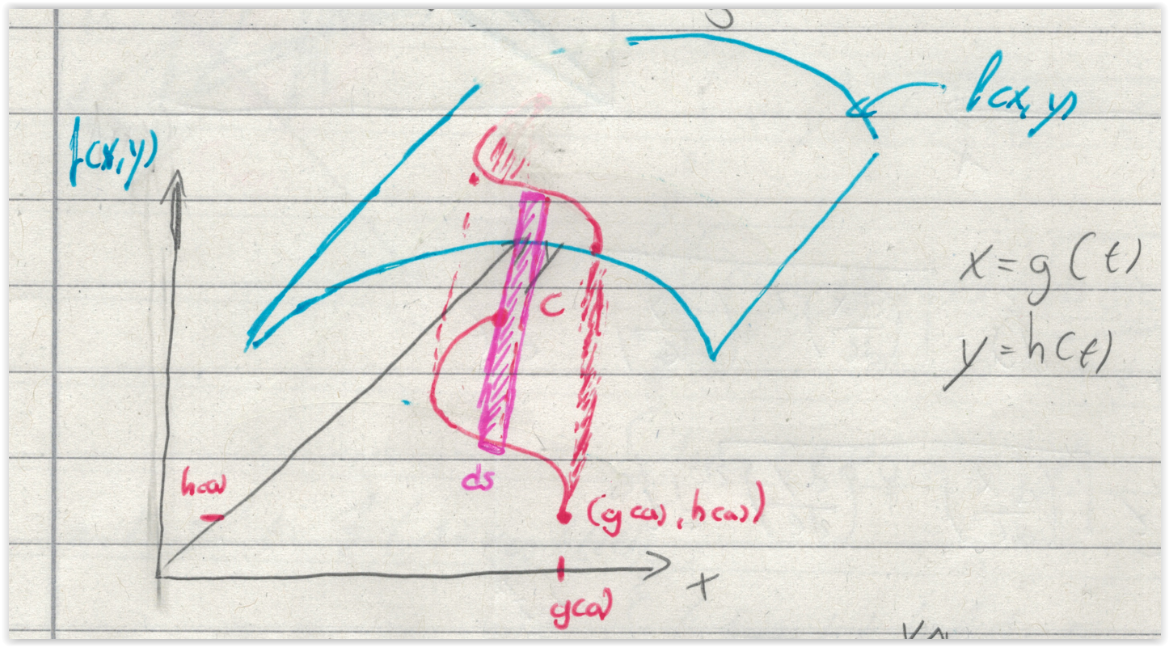
\includegraphics[width=0.9\linewidth]{./img/wegintegral_erster_1.png}
		  \caption{Graphische Interpretation}
		  \label{fig:wegintegral_erster_1}
		\end{minipage}%
		\begin{minipage}{.5\textwidth}
		  \centering
		  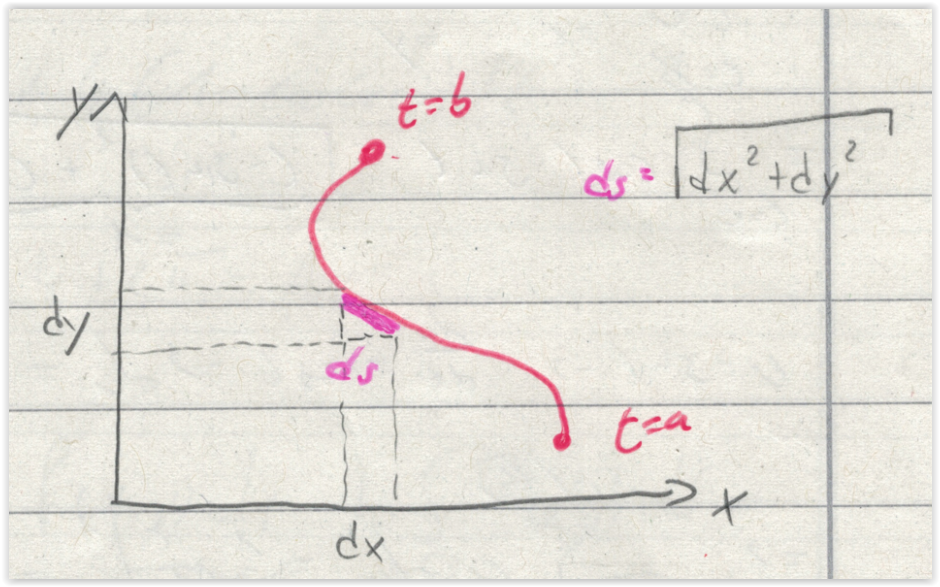
\includegraphics[width=0.8\linewidth]{./img/wegintegral_erster_2.png}
		  \caption{Interpretation von \protect\eqref{eq:wegintegral_1}}
		  \label{fig:wegintegral_erster_2}
		\end{minipage}
		\end{figure}
		\begin{bem}
			\begin{itemize}
			  \item[a) ] Integrale sind unabhängig von der gewählten Parametrisierung.
			  \item[b) ] Falls $c$ geschlossen ist so schreibt man 
				  \begin{equation}
				    \oint\limits_c \varrho \; ds
				  \end{equation}
			\end{itemize}
		\end{bem}
		\subsubsection{Wegintegrale zweiter Art}
		\begin{definition}
		  Sei $f: D\rightarrow \R^d$ ein stetiges Vektorfeld mit $D\subset \R^d$ und sei $c:[a,b] \rightarrow D$ eine stückweise $C^1$-Kurve, dann heißt 
		  \begin{equation}
		    \int\limits_c <f(x), dx> = \int\limits_a^b <f\left(c(t)\right), \dot{c}(t)>dt
		  \end{equation}
		  das Wegintegral 2-ter Art. Falls $c$ geschlossen ist schreibt man
		  \begin{equation}
		    \oint\limits_c <f(x), dx>
		  \end{equation}
		\end{definition}
		\begin{bem}
		  Das Wegintegral ist unabhängig von der gewählten Parametrisierung.
		\end{bem}
		\begin{bem}
		  Eine Alternative ältere Schreibweise ist
		  \begin{equation*}
		    \int\limits_c <f(X),dX>
		  \end{equation*}
		  Achtung, es handelt sich nur um eine Schreibweise. Nicht das Skalarprodukt aus $f(X)$ und $dX$ bilden!
		\end{bem}
		\begin{definition}
  		Ein stetiges Vektorfeld $f$ heißt wirbelfrei, falls die Kurvenintegrale längs aller stückweise stetig diffbaren Kurven verschwinden, d.h.
  		\begin{equation}
  		  \oint\limits_c <f(x), dx> = 0
  		\end{equation}
  		gilt.
		\end{definition}
		Als Konsequenz daraus folgt die Wegunabhängigkeit der Kurvenintegrale für den Fall das $f$ wirbelfrei ist. Das heißt, ist $f$ wirbelfrei, so gilt:
		\begin{equation}
		  \int\limits_{c_1} <f(x),dx> = \int\limits_{c_2} <f(x),dx>
		\end{equation}
		für beliebige Wege $c_1$ und $c_2$ mit gleichen Anfangs- und Endpunkten.
		\begin{definition}
		  Eine Teilmenge $D \subset \R^d$ heißt (weg)-zusammenhängend, falls je zwei Punkte $x,y \in D$ durch eine stückweise $C^1$-Kurve in $D$ verbunden werden können.
		  \begin{figure}[H] 
			  \centering
			  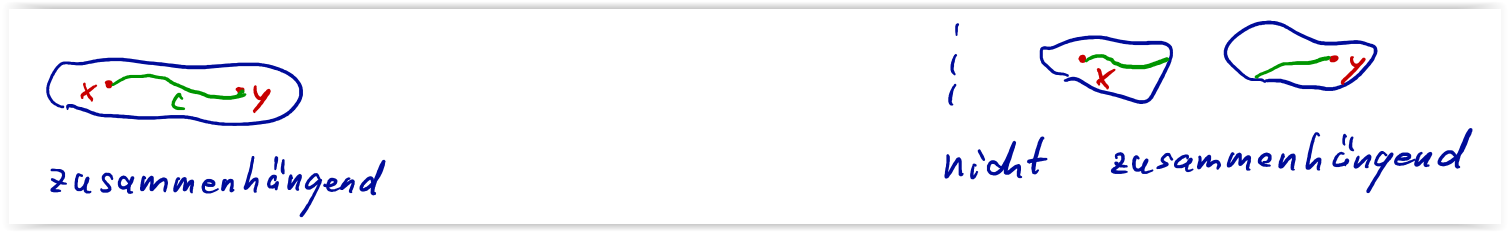
\includegraphics[width=0.8\linewidth]{./img/zusammenhaengend.png}
			  \caption{Visualisierung zusammenhängend \protect\cite{HM12}}
			  \label{fig:zusammenhängend}
		  \end{figure}
		\end{definition}
		\subsubsection{Potential}
	  \begin{definition}
	    Sei $f:D\rightarrow \R^d$ ein Vektorfeld auf $D\subset \R^d$. Wir sagen $f$ ist ein gradientenfeld, falls es eine skalare $C^1$-Funktion $\varphi: D\rightarrow\R$ gibt, mit 
	    \begin{equation}
	    \nabla \varphi(x) = f(x)
	    \end{equation}
	    $\varphi$ heißt das Potential von $f$.
	  \end{definition}
    \begin{satz}
      Sei $D \subset \R^n$ offen und zusammenhängend und $f$ ein stetiges Vektorfeld auf $D$. 
      \begin{itemize}
        \item[a) ] Besitzt $f$ ein Potential $\varphi$, so gilt für alle stückweisen $C^1$-Kurven $c$, dass 
        \begin{equation}
          \int\limits_c <f(x),dx> = \varphi(c(b)) - \varphi(c(a))
        \end{equation}
        wobei $c:[a,b]\rightarrow \R^d$. D.h. das Wegintegral ist damit wegunabhängig und $f$ wirbelfrei.
        \item[b) ] Ist $f$ wirbelfrei, so besitzt $f$ ein Potential $\varphi$ mit der Darstellung 
        \begin{equation}
          \varphi(x) = \int\limits_{c_x} <f(\tilde{x}),d\tilde{x}>
        \end{equation}
        wobei $c_x$ ein Weg nach $x$ mit fest gewähltem Startpunkt $x^*$ sein soll.
      \end{itemize}
    \end{satz}	  
	  \subsubsubsection{Berechnung von Potentialen}
	  Die notwendige (aber nicht hinreichende) Bedingung für die Existenz eines Potentials ist:
	  \begin{equation}
	    rot(\nabla \varphi) = 0 \Rightarrow rot(f) = 0 \Rightarrow Potential\;ex.  
	  \end{equation}
	  \begin{definition}
	    Ein Gebiet $G$ heißt einfach zusammenhängend, falls jeder geschlossene Weg in $G$ auf einen Punkt im Gebiet zusammen gezogen werden kann.
	    \begin{figure}[H] 
			  \centering
			  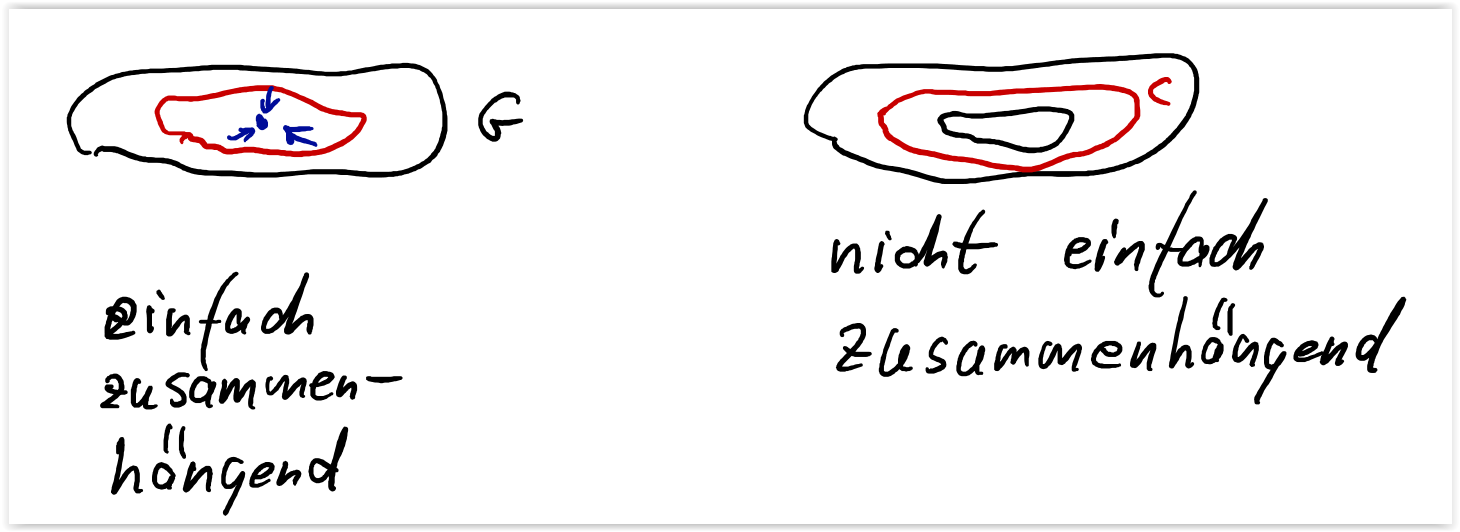
\includegraphics[width=0.8\linewidth]{./img/einfach_zusammenhaengend.png}
			  \caption{Visualisierung einfach zusammenhängend \protect\cite{HM12}}
			  \label{fig:einfach_zusammenhängend}
		  \end{figure}
	  \end{definition}
	\subsection{Definitionen}
	\subsubsection{2D-Divergenz}
	\begin{equation}
		\diverg \vec{F}(x,y) = \lim_{|A_(x,y)|\to 0} \underbrace{\frac{1}{|A_{(x,y)}|} \overbrace{\oint_c \vec{F} \vec{n}\;ds}^{\text{2d-Fluss}}}_{\text{Fluss pro Flächeneinheit}}
	\end{equation}
	\subsubsection{3D-Divergenz}
	\begin{equation}
		\diverg \vec{F}(x,y,z) = \lim_{R \to (x,y,z)}\frac{1}{|R|} \int \int_s \vec{F} \vec{n}\;ds
	\end{equation}
	\subsubsection{2D-Rotation}
	\begin{equation}
		\rot_2 \vec{F}(x,y) = \lim_{A_(x,y)\to 0} \underbrace{\frac{1}{|A_{(x,y)}|}\oint_c \vec{F} \;dr}_{\text{durchschnittliche Rotation pro Flächeneinheit}}
	\end{equation}
	\subsubsection{3D-Rotation}
	\begin{equation}
		\rot \vec{F}(x,y) \cdot \hat{e}_x = \lim_{|A_{(x,y,z)},\hat{e}_x \to 0} \frac{1}{|A_{(x,y,z)},\hat{e}|}\oint_c \vec{F} \;dr
	\end{equation}
	Analog für $\hat{e}_y$ und $\hat{e}_z$.
	
	\subsection{Satz von Green}
	Sei $f$ ein $C^1$-Vektorfeld, $D \subset \R^2$ offen und zusammenhängend. $K \subset D$ sei komplett und bezüglich beider Koordinatenrichtungen ein Normalbereich. $K$ werde von einer $C^1$-Kurve $c:t\to c(t)$ berandet. Die Parametrisierung sei  so gewählt, dass $K$ linkgs von der Durchlaufrichtung liegt. Dann gilt
	\begin{equation}
		\oint_c < \underbrace{f(\vec{x})}_{\in \R^2}, \underbrace{d\vec{x}>}_{\in \R^2} = \int_K rot_2 f(\vec{x}) \; d\vec{x}
	\end{equation}		
	Und es ist
	\begin{equation}
		\rot_2 f(\vec{x}) = \frac{\partial f_2}{\partial x_1} - \frac{\partial f_1}{\partial x_2}
	\end{equation}
	  \begin{figure}[H] 
		  \centering
		  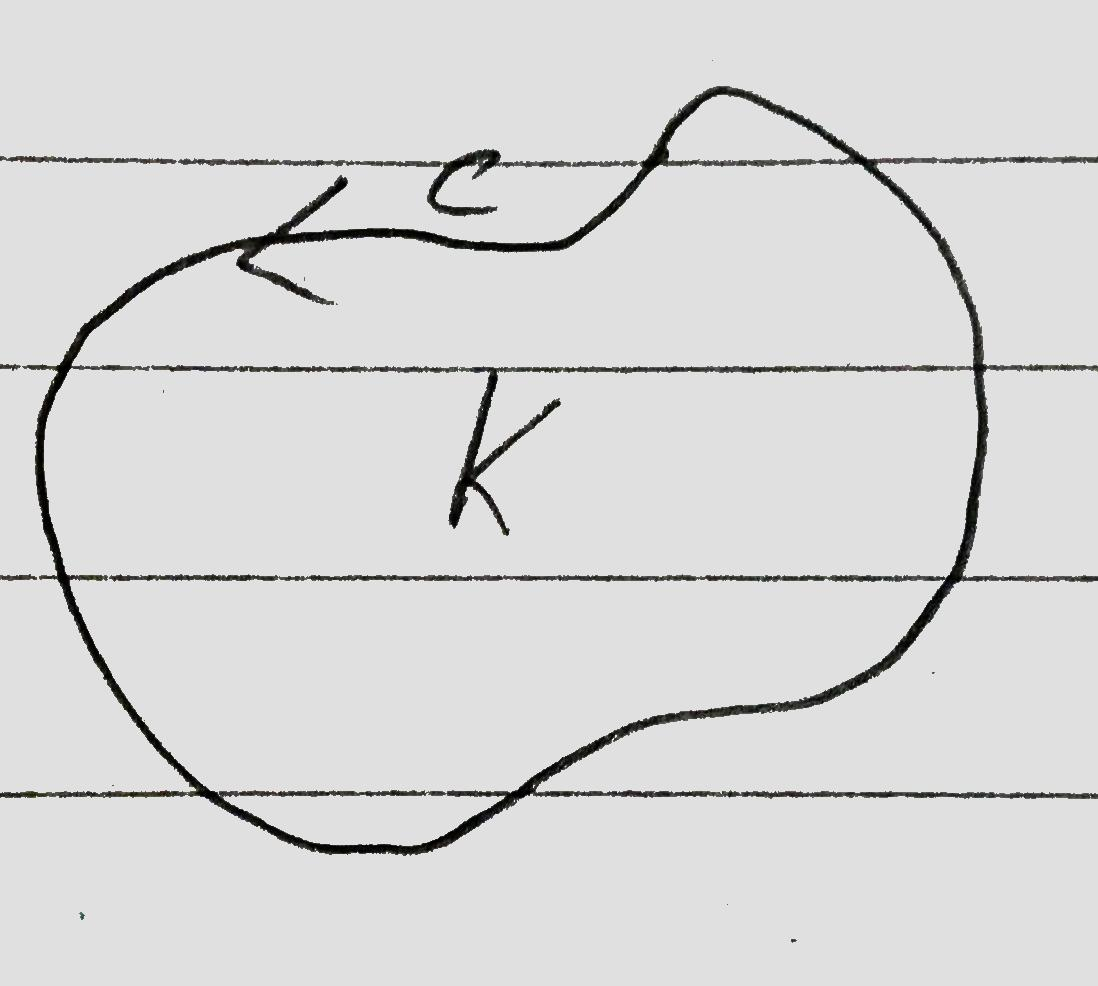
\includegraphics[width=0.25\textwidth]{./img/green_a.jpg}
		  \caption{Durchlaufrichtung}
		  \label{fig:green_a}
	  \end{figure}
	  \begin{bem}
	  	Ist $K\subset \R^2$ ein regulärer Bereich, dann gilt
	  	\begin{equation}
	  		v(K) = \int_{\partial K} x \dy = - \int_{\partial K} y \dx
	  	\end{equation}
	  \end{bem}
	  
	\subsection{Satz von Gauss}
	\subsubsection{Überleitung}
	Der Fluss über den Rand im $\R^2$ ist gegeben durch
	\begin{equation}
		\underbrace{\int_{\partial R} <\vec{F},\vec{n}>\;dr}_{\text{Fluss über den Rand}} = \underset{R}{\int \int}\diverg \vec{F} \;dA
	\end{equation}
	
	Der Fluss über den Rand im $\R^3$ ist gegeben durch
	\begin{equation}
		\underbrace{\underset{\partial R}{\int \int} <\vec{F},\vec{n}>\;dr}_{\text{Fluss über den Rand}} = \underset{R}{\int \int \int}\diverg \vec{F} \;dV
	\end{equation}
	
	\begin{figure}[H] 
		\centering
		\begin{minipage}{.5\textwidth}
		  \centering
		  \captionsetup{justification=centering}
		 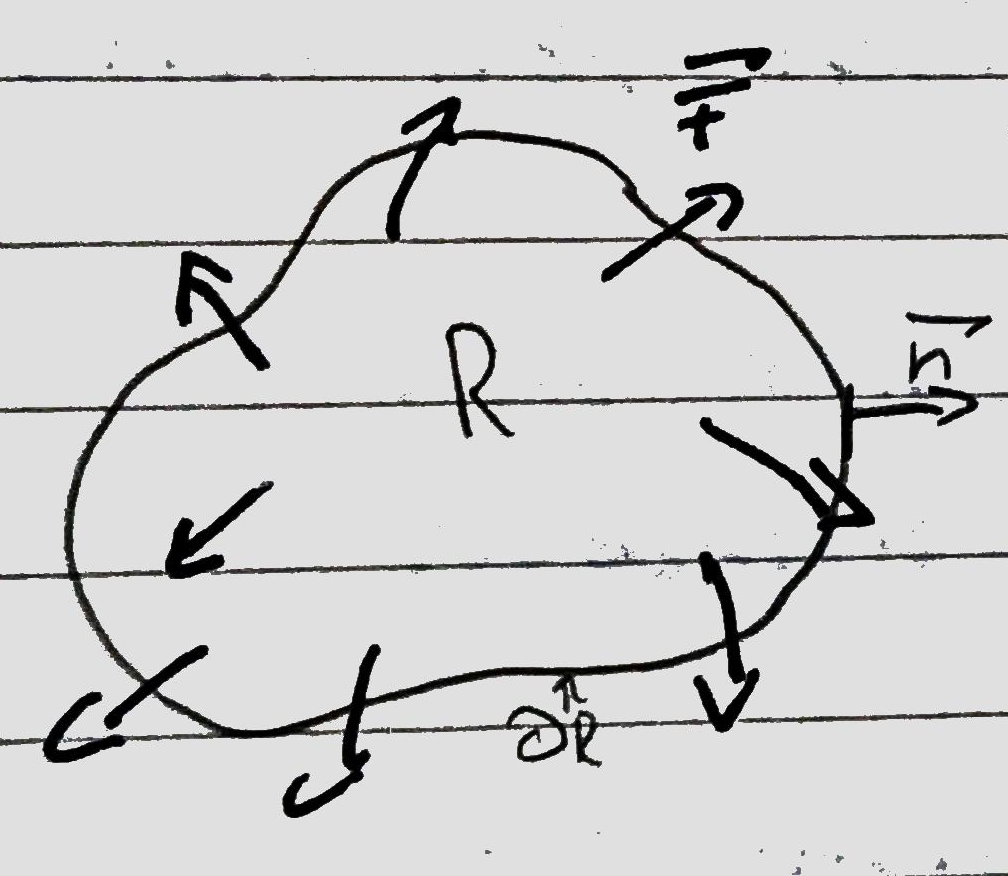
\includegraphics[width=0.6\textwidth]{./img/gauss_a.png}
		  \caption{Fluss über Rand im $\R^2$}
		  \label{fig:gauss_a}
		\end{minipage}%
		\begin{minipage}{.5\textwidth}
		  \centering
		  \captionsetup{justification=centering}
		 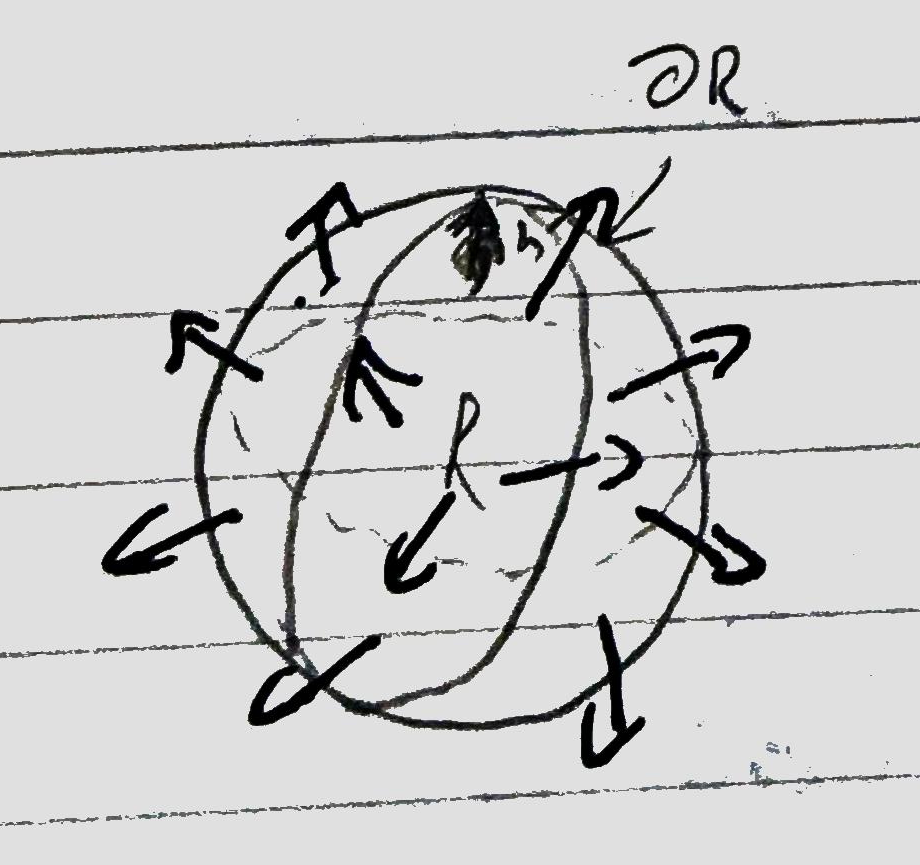
\includegraphics[width=0.55\textwidth]{./img/gauss_b.png}
		  \caption{Fluss über Rand im $\R^3$}
		  \label{fig:gauss_b}
		\end{minipage}
	 \end{figure}
	 
	 \subsubsection{Satz von Gauss (Divergenztheorem)}
	 Ist $B$ ein kompakter Teilbereich des $\R^3$ mit der Oberfläche $\partial B$, die sich auf stückweise stetige Weise parametrisieren lässt, und ist $\vec{v}(\vec{r})$ ein in ganz $B$ stetig differenzierbares Vektorfeld, so gilt, sofern alle vorkommenden Funktionen über die entsprechenden Bereiche integrierbar sind:
	 \begin{equation}
	 	\int_{\partial B} \vec{v} \; \vec{d \sigma} = \int_B \diverg \vec{v} \; d \vec{x}
	 \end{equation}
	 
	 \subsubsection{Satz von Gauss in der Ebene}
	 Für einen kompakten, einfach  zusammenhängenden Bereich $B \subset \R^2$, dessen positiv durchlaufener Rand durch eine stetig diffbare Abbildung $\vec{x} = \vec{x}(t),\;t \in [a,b]$ parametrisiert werden kann, gilt sofern alle beteiligten Funktionen über die entsprechenden Bereiche integrierbar sind
	 \begin{equation}
	 	\int_a^b (v_1(\vec{x}(t)) \frac{dx_2}{dt} - v_2 (\vec{x}(t)) \frac{dx_1}{dt} = \int_B \left( \frac{\partial v_1}{\partial x_1} + \frac{\partial v_2}{\partial x_2}\right) \; d(x_1, x_2)
	 \end{equation}
	 
	 \subsubsection{Satz von Gauss im $R^2$ aus der Vorlesung}
	 Sei $D \subset \R^2$ offen und $\vec{v}:D \to \R^2$ ein $C^1$- Vektofreld. Dann gilt für jeden regulären Bereich $B \subset D$.
	 \begin{equation}
	 	\int_{\partial B} <\vec{v}, \vec{n}>ds =  \int_B \diverg(\vec{v})d(x,y)
	 \end{equation}
	 wobei $|\vec{n}|=1, \vec{n}\perp \partial B$ aus B hinaus zeigt.
	 
	 \subsection{Satz von Stokes}
	 Der Satz von Stokes verknüpft das Kurvenintegral über einen geschlossenen Weg $c$ mit dem Integral der Rotation über eine beliebige von $c$ umrandete Fläche $F$. \newline
	 Für eine orientierbare, stückweise glatte Fläche $F$ mit dem stückweise glatten Rand $\partial F$ und ein auf dem Bild dieser Fläche stetig diffbaren Vektorfeld $\vec{v}$ gilt, sofern alle vorkommenden Funktionen über die entsprechenden Bereiche integrierbar sind
	 \begin{equation}
	 	\oint_{\partial F} \vec{v} \; d\vec{s} = \int_F \rot \vec{v} \; \vec{d \sigma}
	 \end{equation}
	 Dabei ist die Kurve $\partial F$ so parametrisiert, dass sie den nach außen weisenden Normalenvektor $\vec{n} = \frac{\vec{d \sigma}}{d \sigma}$ der Fläche im mathematisch positiven Sinn umläuft.
	 
	 \begin{bem}
	 Einheitsnormalenfeld: Ein Vektorfeld, dass überall auf der Fläche einen Normalenvektor wirken lässt heißt Einheitsnormalenfeld.
	  \begin{figure}[H] 
		  \centering
		  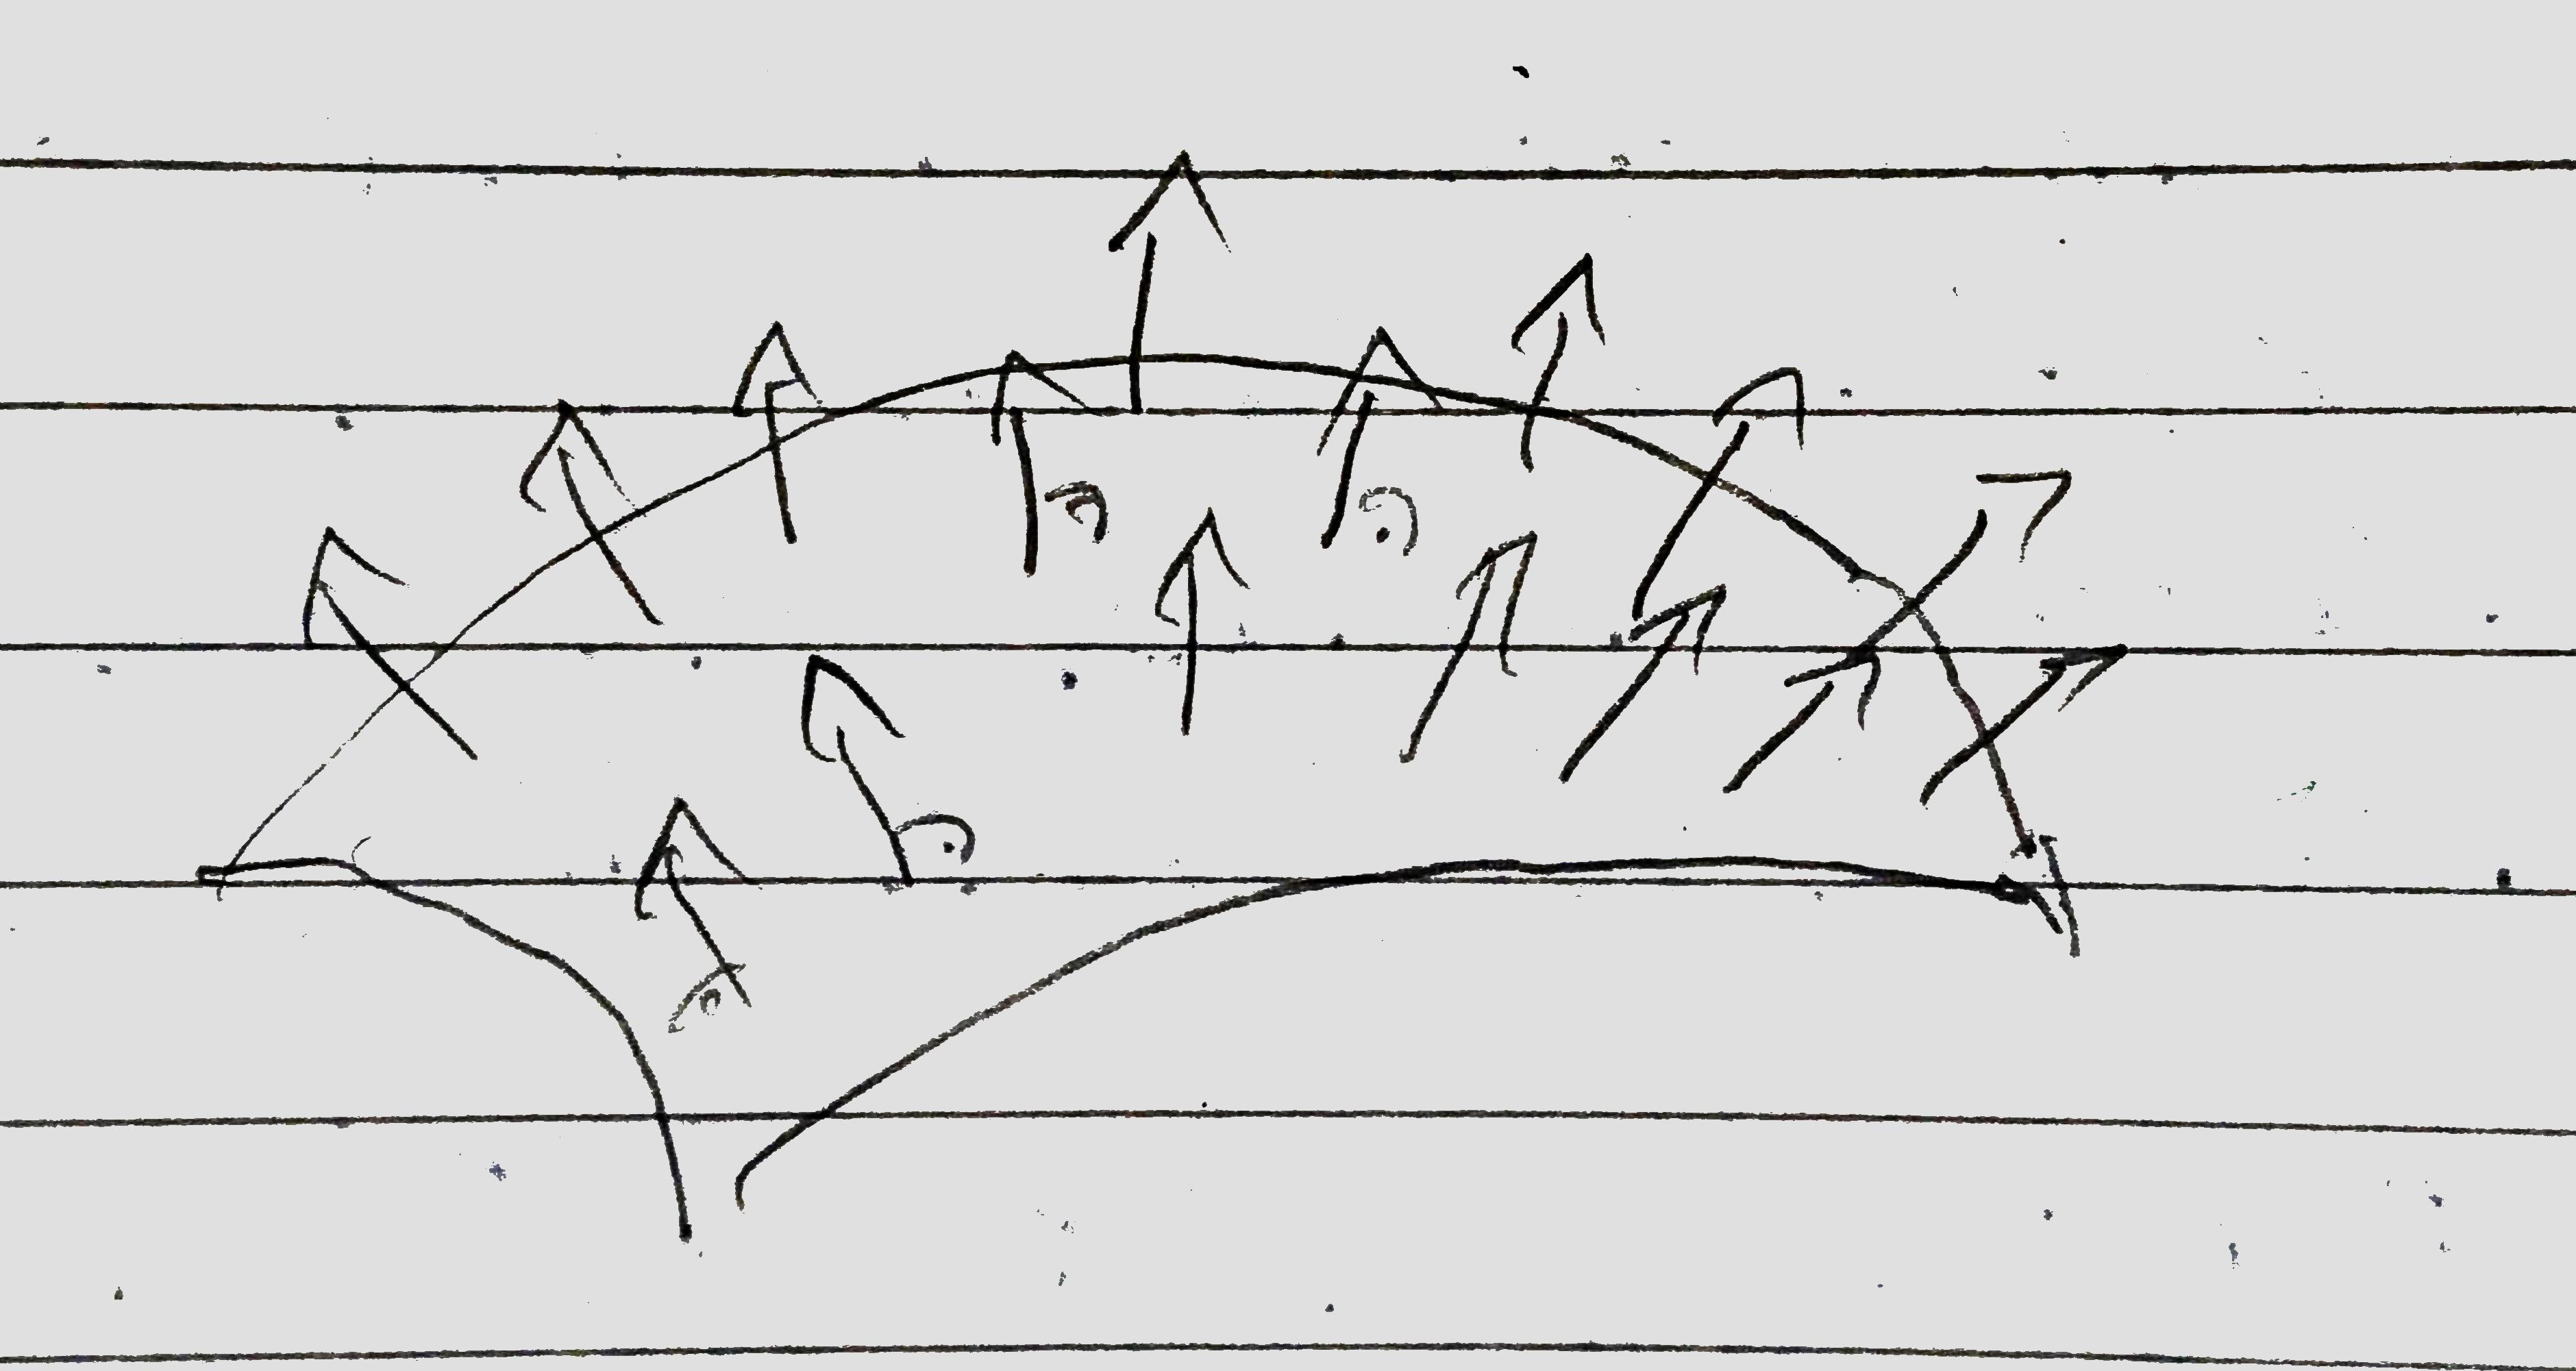
\includegraphics[width=0.5\textwidth]{./img/einheitsnormfeld.png}
		  \caption{Einheitsnormalenfeld}
		  \label{fig:einhNormFeld}
	  \end{figure}
	  \end{bem}
	  %\vspace{-0.5cm}
	  
	  
	  \subsection{Greensche Identität}
	  \begin{equation}
	  	\int_A (f \cdot \lapl g - \lapl f\cdot g)\;d^3 x = \int{\partial A}<f\nabla g - g \nabla f, \vec{n}> d \vec{\sigma}
	  \end{equation}
	  
	  \subsection{Weitere Definitionen}
	  \subsubsection{Regulär}
	  \begin{definition}
	  	Eine Fläche $S \subset \R^3$ heißt stückweise regulär, wenn sie zusammengesetzt ist aus endlich vielen regulären Flächenstücken $s_1 ... s_n$:
	  	\begin{equation}
	  		S = \sum_{i = 1}^n s_i
	  	\end{equation}
	  	wobei sich nur die Ränder berühren dürfen. Der Rand $\partial S$ von $S$ besteht dann per Definition aus allen Randstücken $\partial s_i$ die nur zu einem $s_i$ gehören.
	  \end{definition}
	  
	  